%% The following is a directive for TeXShop to indicate the main file
%%!TEX root = diss.tex

\chapter{Lexical decision}

This chapter reports on two experiments done using a lexical decision paradigm to induce auditory perceptual learning in participants.  This paradigm has been most used in the previous literature (Reinisch line of work, McQueen line of work, some kraljic? but I think some other kraljic uses shapes - maybe just for unlearning phase).

\section{Motivation}

\subsection{Perceptual learning}

A listener's perceptual system shifts rapidly; for instance, vowel perception can shift solely on the basis of the vowels in a  preceding sentence \citep{Ladefoged1957}.  Boundaries between fricative categories can be changed by exposure to relatively small amount of ambiguous fricative tokens, but they must be embedded within and associated with a lexical item in a language, and hearing ambiguous productions between two sound categories in nonwords does not induce perceptual learning \citep{Norris2003}. However, besides the categorical distinction separating words from nonwords, little is known about the factors that influence linking an shifted or ambiguous production of a sound with a category through a lexical item. My dissertation investigates the factors which can contribute to associating ambiguous atypical productions with a specific sound category through lexical items. 

Given a continuum from a nonword like \emph{dask} to word like \emph{task} that differs only in one sound, listeners in general are more likely to interpret any step along the continuum as the word endpoint rather than the nonword endpoint \citep{Ganong1980}. This lexical bias, also know as the Ganong effect, is exploited in perceptual learning studies to allow for noncanonical, ambiguous productions of a sound to be linked to pre-existing sound categories.

\subsection{Lexical bias}

Lexical bias, however, has been shown to be gradient.  When an ambiguous sound is embedded later in a word, listeners are more likely to treat the production as a word than if the same sound is embedded earlier in the word \citep{Pitt2012}.  The same study found that when listeners are alerted to the ambiguous sound's presence, and told to listen carefully, lexical biases diminish overall, with listeners less likely to treat the production as a word.    Most studies looking at boundaries between fricative categories use longer (2-3 syllable) lexical items ending with a fricative \citep{Norris2003}, but perceptual learning has also been found following exposure to shorter (1 syllable) lexical items beginning with an ambiguous sound \citep{Clare2014}.  However, specific comparisons in perceptual learning effects across word position in these studies is impossible due to differences in languages under investigation (Dutch or English) and the nature of contrast (/t/-/d/, /s/-/sh/, or /s/-/f/). Studies also differ on the ambiguity of the sound, with some attempting to control for the Ganong effect by picking an ambiguous sound farther away from the more canonical word form \citep{Reinisch2013} and some selecting a production halfway in between word and nonword \citep{Norris2003}.  The first two experiments in my dissertation address this gap in the literature and investigate the mechanism underlying perceptual learning.

Given the difference in word response rates depending on position in the word, we would predict that listeners exposed to ambiguous sounds earlier in words would be less likely to accept these productions as words as compared to listeners exposed to ambiguous sounds later in words.  In addition, given the reliance of perceptual learning on lexical scaffolding, this lower acceptance rate for the former group would lead to a smaller perceptual learning effect as compared to the latter group.

In these two experiments, listeners will be exposed to ambiguous productions of words containing a single instance of /s/, where the /s/ has been modified to sound more like /sh/ in a lexical decision task.  In one group, the S-Initial group, the critical words will have an /s/ in the onset of the first syllable, like in \emph{cement}, with no /sh/ neighbour, like \emph{shement}.  In the other group, the S-Final group, the critical words will have an /s/ in the onset of the final syllable, like in \emph{tassel}, with no /sh/ neighbour like \emph{tashel}.  In addition, half of each group will be given instructions that the speaker has a ambiguous /s/ and to listen carefully, following \citet{Pitt2012}.

The two experiments differ in the salience of the ambiguous stimuli, with salience here defined as the distance from a normal, natural production.  A pretest was conducted with 20 listeners to determine the percentage /s/ response at each step of the critical continua (for instance, from \emph{tassel} to \emph{tashel}).  In the first experiment, the continua steps selected for the critical item  were around 30\% /s/ response, following \citet{Reinisch2013}.  In the second experiment, the continua steps selected for critical items were around 50\% /s/ response, following other methodologies \citep{Norris2003,Kraljic2005}, which should be more susceptible to lexical biases.  The differences in perceptual learning between the groups are predicted be less in the first experiment than in second, as the lessened salience of the stimuli in the second experiment is predicted to allow for a greater role of top-down attention on the processing of the exposure items.

\section{Experiment 1}

\subsection{Methodology}

\subsubsection{Participants}

One hundred native speakers of English (mean age ??, range ??-??) participated in the experiment and were compensated with either \$10 CAD or course credit. They were recruited from the UBC student population.  Twenty additional native English speakers participated in a pretest to determine the most ambiguous sounds.  Twenty five other native speakers of English participated for course credit in a control experiment.

\subsubsection{Materials}

One hundred and forty English words and 100 nonwords that were phonologically legal in English were used as exposure materials.  The set of words consisted of 40 critical items, 20 control items and 60 filler words.  Half of the critical items had an /s/ in the onset of the first syllable and half had an /s/ in the onset of the final syllable.  All critical tokens formed nonwords if their /s/ was replaced with /sh/. Half the control items had an /sh/ in the onset of the first syllable and half had an /sh/ in the onset of the final syllable.  Each critical item and control item contained just the one sibilant, with no other /s z sh zh ch or jh/.  Filler words and nonwords did not contain any sibilants.  Four monosyllabic minimal pairs of voiceless sibilants were selected as test items for categorization (\emph{sack}-\emph{shack}, \emph{sigh}-\emph{shy}, \emph{sin}-\emph{shin}, and \emph{sock}-\emph{shock}).  Two of the pairs had a higher log frequency per million words (LFPM) from SUBTLEXus (cite) for the /s/ word, and two had higher LFPM for the /sh/ word.  \emph{Sack}-\emph{shack} had frequencies of 1.11  LFPM and 0.75  LFPM, \emph{sigh}-\emph{shy} had frequencies of 0.53  LFPM and 1.26  LFPM, \emph{sin}-\emph{shin} had frequencies of 1.20  LFPM and 0.48  LFPM, and \emph{sock}-\emph{shock} had frequencies of 0.95  LFPM and 1.46 LFPM.

All words and nonwords were recorded by a male Vancouver English speaker in quiet room.  Critical words for the exposure phase were recorded in pairs, once normally and once with the sibilant swapped forming a nonword.  The speaker was instructed to produce both forms with comparable speech rate, speech style and prosody.

For each critical item, the word and nonword versions were morphed together in an 11-step continuum (0\%-100\% of the nonword /sh/ recording, in steps of 10\%) using STRAIGHT (cite) in Matlab (cite).  Prior to morphing, the word and nonword versions were time aligned based on acoustic landmarks, like stop bursts, onset of F2, nasalization or frication, etc.  All control items and filler words were processed and resynthesized by STRAIGHT to ensure a consistent quality across stimulus items.

\subsubsection{Pretest}

To determine which step of each continua would be used in exposure, a phonetic categorization experiment was conducted.  Participants were presented with each step of each exposure word-nonword continuum and each categorization minimal pair continuum, resulting in 495 trials (40 exposure words plus five minimals pairs by 11 steps).  The experiment was implemented in E-prime (cite).  As half of the critical items had a sibilant in the middle of the word (onset of the final syllable), participants were asked to respond with word or non word rather than asking for the identity of the ambiguous sound, as in previous research \citep{Reinisch2013}.  

\begin{figure}
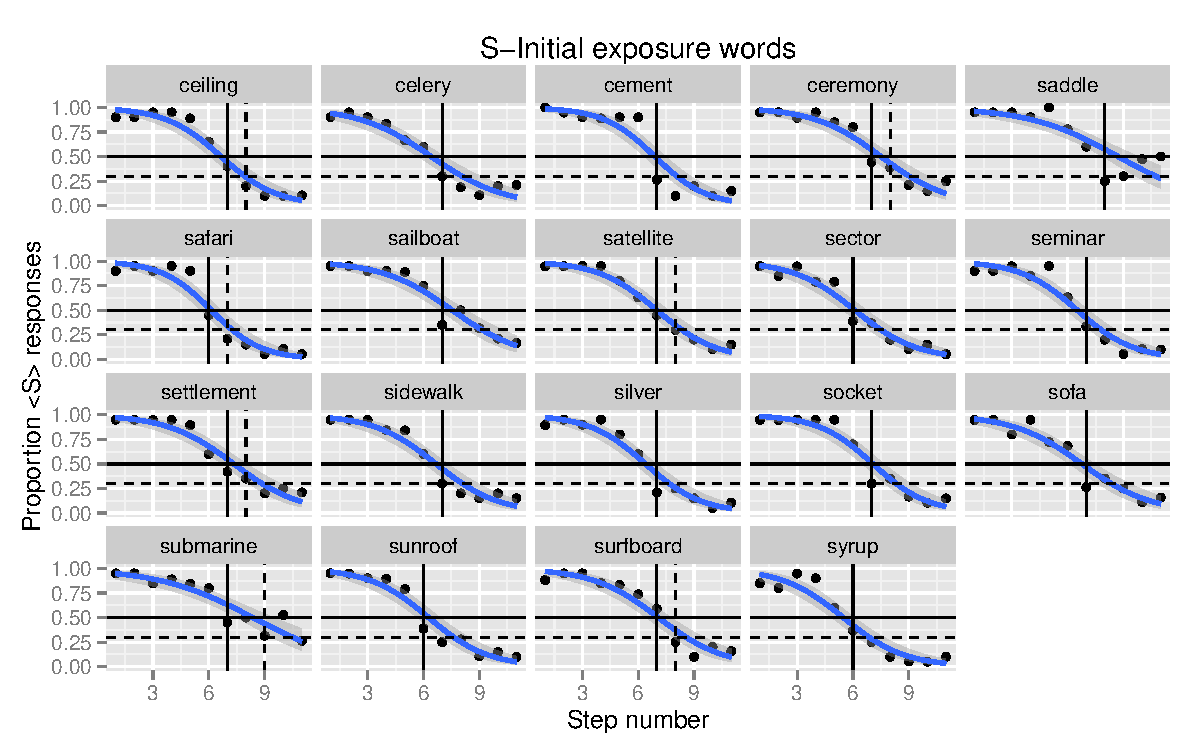
\includegraphics[width=\textwidth]{sinitialpretest.pdf}
\caption{Proportion of word-responses for /s/-initial exposure words. Solid lines represent Experiment 1 selection criteria (50\% word-response rate) and dashed lines represent Experiment 2 selection criteria (30\% word-response rate).  Dots are averaged word-response across subjects, and the blue line is a binomial model constructed from the responses.}
\end{figure}

The proportion of s-responses (or word responses for exposure items) at each step of each continuum was calculated and the most ambiguous step chosen.  The threshold for the ambiguous step for this experiment was when the percentage of s-response dropped near 50\%. A full list of steps chosen for each stimulus item is in the appendix.  For the minimal pairs, six steps surrounding the 50\% cross over point were selected for use in the phonetic categorization task.  Due to experimenter error, the continuum for \emph{seedling} was not included in the stimuli, so the chosen step was the average chosen step for the /s/-initial words.  The average step chosen for /s/-initial words was 6.8 ($SD = 0.5$), and for /s/-final words the average step was 7.7 ($SD = 0.8$).

\begin{figure}
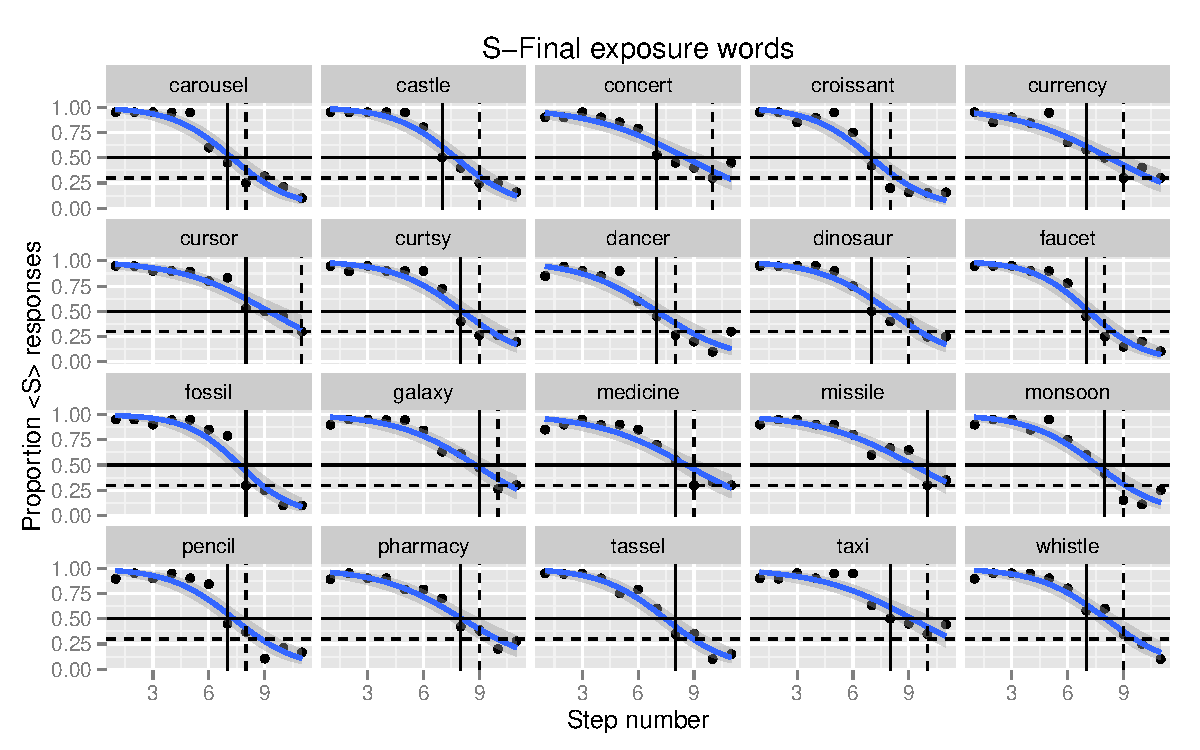
\includegraphics[width=\textwidth]{sfinalpretest.pdf}
\caption{Proportion of word-responses for /s/-final exposure words. Solid lines represent Experiment 1 selection criteria (50\% word-response rate) and dashed lines represent Experiment 2 selection criteria (30\% word-response rate).  Dots are averaged word-response across subjects, and the blue line is a binomial model constructed from the responses}
\end{figure}

\subsubsection{Procedure}

Participants in the experimental conditions completed two tasks, an exposure task and a categorization task.  The exposure task was a lexical decision task, where participants heard auditory stimuli and were instructed to respond with either "word" if they thought what they heard was a word or "nonword" if they didn't think it was a word.  The buttons corresponding to "word" and "nonword" were counterbalanced across participants. Trial order was pseudorandom, with no critical or control items appearing in the first six trials, and no critical or control trials in a row, but random otherwise, following (ReinischWeberMitter2012).

In the categorization task, participants heard an auditory stimulus and had to categorize it as one of two words, differing only in the onset sibilant (s vs sh).  The buttons corresponding to the words were counterbalanced across participants.  The six most ambiguous steps of the minimal pair continua were used with seven repetitions each, giving a total of 168 trials. Participants were instructed that there would two tasks in the experiment, and both tasks were explained at the beginning to remove experimenter interaction between exposure and categorization.  

Participants were assigned to one of four conditions.  Two of the conditions exposed participants to only criticall items that began with /s/, and the other two exposed them to only critical items that had an /s/ in the onset of the final syllable, giving a consistent 200 trials in all exposure phases with control and filler items shared across all participants.  Additionally participants in half the conditions received additional instructions that the speaker's "s" sounds were sometimes ambiguous, and to listen carefully to ensure correct responses in the lexical decision.

\subsection{Results}

\subsection{Discussion}

\section{Experiment 2}

\subsection{Methodology}

This experiment followed an identical methodology as experiment 1, except that the step along the /s/-/sh/ continua chosen as the ambiguous sound had a different threshold.  For this experiment, 30\% identification as the /s/ word was used the threshold. The average step chosen for /s/-initial words was 7.3 ($SD = 0.8$), and for /s/-final words the average step was 8.9 ($SD = 0.9$).

\subsection{Results}

\subsection{Discussion}